\subsubsection{Net 6}
 
\zadatak Koje vrednosti zadovo{\lj}avaju uslov
\begin{align*}
\log_2(x+1) &> \log_4x^2?
\intertext{\resenje Ako levu stranu zapi{\sv}emo kao}
2\cdot\frac12\log_2(x+1)&=\log_{2^2}(x+1)^2 
\intertext{{\sv}to sledi iz jednakosti \eqref{eq:powbase} i \eqref{eq:bpow},
dobi{\cc}emo}
\log_4 (x+1)^2 &> \log_4 x^2\\
(x+1)^2 &> x^2\\
x^2+2x+1&> x^2\\
2x+1&>0\\
x&>-\frac12.
\end{align*}
Kako mora da va{\zv}i $x>-1$ i $x\ne0$, dobijamo kona{\cv}no re{\sv}e{\nj}e
$$
    x\in\ram{\left({-\frac12},0\right)\cup(0,\infty)}.    
$$
$$
\slika{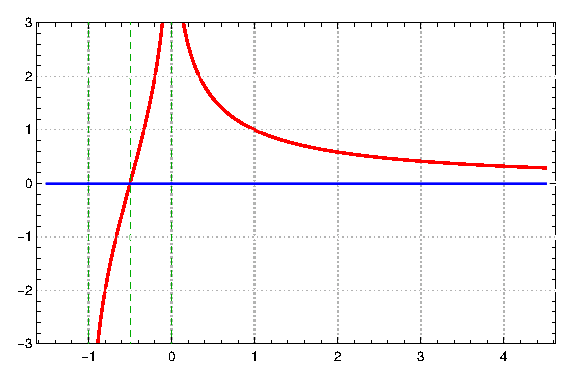
\includegraphics[width=\sirina]{eps/net6.eps}}{$y=\log_2 (x + 1)-\log_4 x^2$.}
$$

\dodatak Kao {\sv}to je na strani \pageref{danger} napomenuto, 
da smo $\log_4 x^2$ jednostavno predstavili kao $\log_{2^2}x^2=\log_2 x$,
dobili bismo neta{\cv}no re{\sv}e{\nj}e. Ispravno bi bilo $\log_4 x^2=\log_2|x|$,
kada bismo posebno gledali 2 slu{\cv}aja: za $x>0$ i za $x<0$.
